\chapter{Results and Discussion}\label{ch:results}

This chapter reports the experimental results. Section~\ref{sec:setup} recalls
the setup, Sections~\ref{sec:detectionresults}--\ref{sec:classresults} present
pair detection, similarity structure, threshold sensitivity, and relationship
classification, Section~\ref{sec:agreementresults} covers the ground-truth
validation study, and Sections~\ref{sec:efficiency}--\ref{sec:threats} discuss
the findings against the research questions and the threats to their validity.

\section{Experimental setup}\label{sec:setup}

All eleven methods were run on the full cross product of 69 \standardA{}
provisions and 72 \standardB{} provisions (4{,}968 pairs) and evaluated on
the 107 annotated pairs: 85 related pairs and 22 annotated negatives
(Figure~\ref{fig:gtdist}). The distribution is dominated by \textsc{Overlap}
(51 pairs), with \textsc{Equivalence} rare (3 pairs) --- the two standards
describe different system layers, so identical requirements barely occur.
Metrics outside the annotated scope are not computable and are not claimed.

\begin{figure}[htbp]
\centering
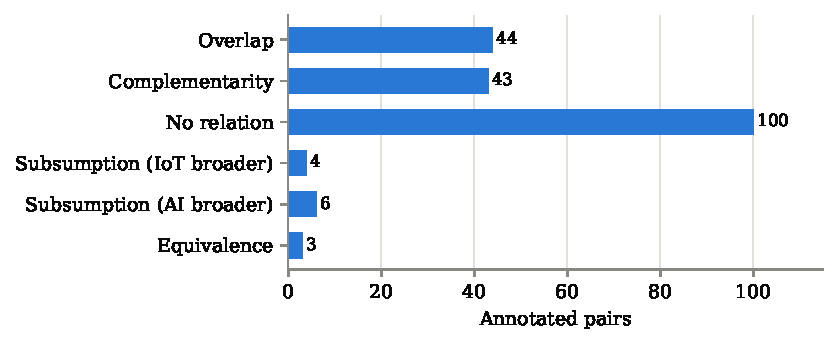
\includegraphics[width=0.72\textwidth]{figures/gt_distribution}
\caption{Distribution of relationship labels in the 107-pair ground truth.}
\label{fig:gtdist}
\end{figure}

\section{Pair detection}\label{sec:detectionresults}

Table~\ref{tab:detection} and Figure~\ref{fig:detectionbars} show the
detection results; Figure~\ref{fig:cis} adds bootstrap confidence intervals.

\begin{table}[htbp]
\centering
\caption{Pair detection on the annotated scope. $P^{+}$ is the number of
pairs the method marks as related among the 107 annotated pairs. Precision
counts false positives only on the 22 annotated negatives, which is why
sparse methods show precision 1.00 despite very low recall.}
\label{tab:detection}
\small
\begin{tabular}{lrrrrrrr}
\toprule
Method & $P^{+}$ & TP & FP & FN & Precision & Recall & F1\\
\midrule
TF--IDF            &   3 &  3 &  0 & 82 & 1.000 & 0.035 & 0.068\\
Keyword Jaccard    &   6 &  6 &  0 & 79 & 1.000 & 0.071 & 0.132\\
Sentence-BERT      &  15 & 15 &  0 & 70 & 1.000 & 0.176 & 0.300\\
MPNet              &  14 & 14 &  0 & 71 & 1.000 & 0.165 & 0.283\\
BGE                &  90 & 75 & 15 & 10 & 0.833 & 0.882 & 0.857\\
BERT               & 105 & 85 & 20 &  0 & 0.809 & 1.000 & \textbf{0.895}\\
SecureBERT         & 107 & 85 & 22 &  0 & 0.794 & 1.000 & 0.885\\
CySecBERT          & 107 & 85 & 22 &  0 & 0.794 & 1.000 & 0.885\\
NLI cross-encoder  &   5 &  5 &  0 & 80 & 1.000 & 0.059 & 0.111\\
Gemini embeddings  & 107 & 85 & 22 &  0 & 0.794 & 1.000 & 0.885\\
Gemini LLM         &  94 & 73 & 21 & 12 & 0.777 & 0.859 & 0.816\\
\bottomrule
\end{tabular}
\end{table}

\begin{figure}[htbp]
\centering
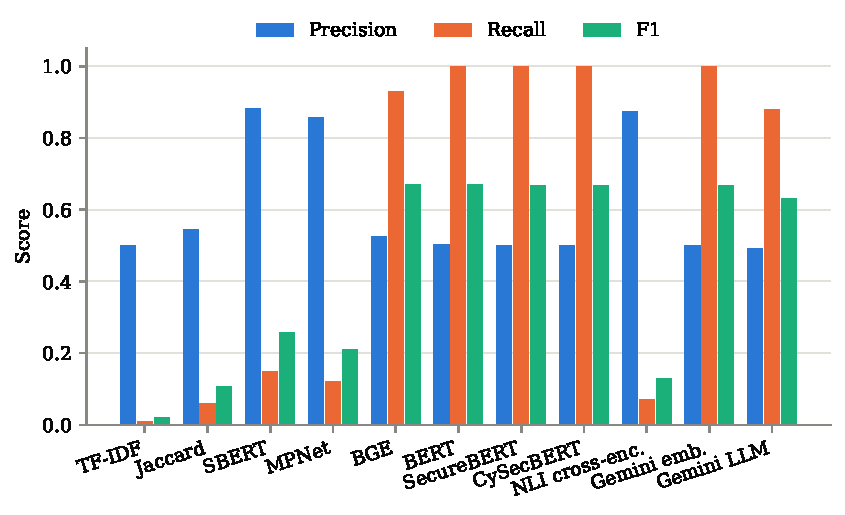
\includegraphics[width=0.9\textwidth]{figures/detection_metrics}
\caption{Pair-detection precision, recall, and F1 per method.}
\label{fig:detectionbars}
\end{figure}

\begin{figure}[htbp]
\centering
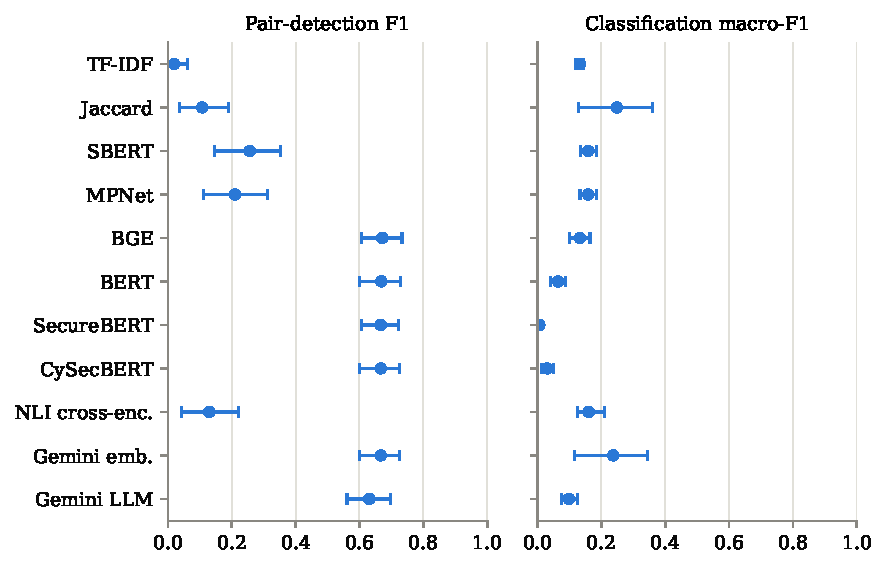
\includegraphics[width=\textwidth]{figures/f1_confidence_intervals}
\caption{Bootstrap 95\% confidence intervals (2{,}000 resamples) for
pair-detection F1 and classification macro-F1.}
\label{fig:cis}
\end{figure}

The table splits the methods into two regimes. The lexical baselines and
Sentence-BERT at its default operating point predict very few relations; what
they do predict is correct (no false positives), but recall between 0.02 and
0.17 makes them useless as stand-alone detectors. The remaining methods sit at
the opposite extreme. SecureBERT and Gemini embeddings mark \emph{every}
annotated pair as related, and BERT marks all but two. Their high F1
($\approx$0.89) must therefore be read with care: with 85 of 107 annotated
pairs being positives, the trivial strategy ``call everything related''
already achieves F1 = 0.885. BERT, SecureBERT, and Gemini embeddings
essentially implement that strategy, and the Gemini LLM (F1 = 0.816) stays
below it. Detection F1 within the annotated scope, in other words, barely
distinguishes these methods; the informative differences appear in the
similarity structure and in classification.

\section{Similarity structure}\label{sec:simstructure}

\begin{figure}[htbp]
\centering
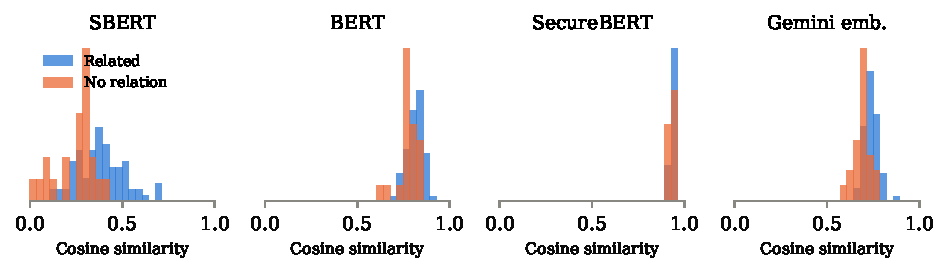
\includegraphics[width=\textwidth]{figures/similarity_distributions}
\caption{Score distributions for annotated related pairs (blue) and annotated
negatives (orange), one panel per method with a continuous score. Panels are
not on a common scale: what matters is the separation between the two
distributions within a panel, not where either sits.}
\label{fig:simdist}
\end{figure}

Figure~\ref{fig:simdist} explains the degenerate behaviour, and with eleven
methods the pattern is legible as a family property rather than a quirk of one
model. All three contextual-embedding models compress: BERT places every pair,
related or not, between roughly 0.57 and 0.91; CySecBERT between 0.71 and 0.93;
SecureBERT is the extreme case, packing the entire corpus into
$[0.875, 0.971]$, a band 0.10 wide. With ranges that narrow, the fixed label
thresholds of Section~\ref{sec:thresholds} land every pair in the same band:
SecureBERT assigns \textsc{Equivalence} to all 4{,}968 possible pairs, and
CySecBERT splits them between \textsc{Equivalence} and \textsc{Overlap} without
ever reaching \textsc{No relation}. This matches the known anisotropy of
contextual embedding spaces~\cite{ethayarajh2019contextual}: mean-pooled vectors
from models never trained for sentence similarity crowd into a narrow cone, and
cosine similarity loses its discriminative meaning. Adding cybersecurity
vocabulary does not repair the geometry --- both domain-adapted models are more
compressed than the general-purpose model they descend from, not less.

The sentence-embedding models spread out, as their training intends.
Sentence-BERT and MPNet span roughly $[-0.05, 0.8]$ and visibly separate the two
distributions --- yet even there the overlap is substantial, confirming that
annotated negatives (chosen to share surface vocabulary) are genuinely hard.
BGE is the instructive intermediate: it is trained for similarity and separates
the classes well, but its scores never fall below 0.345, so a threshold chosen
for its family lands beneath its entire distribution. Its saturation is an
artefact of where its scores sit, not of what they encode --- which is exactly
the distinction the recalibration in Section~\ref{sec:prevalence} isolates.
Gemini embeddings sit between the extremes: compressed range, but with related
pairs shifted consistently above negatives. The NLI cross-encoder is unlike all
of them, producing a probability rather than a cosine and placing the bulk of
pairs near zero, which is why its panel looks empty on the right.

\section{Threshold sensitivity}\label{sec:thresholdresults}

\begin{figure}[htbp]
\centering
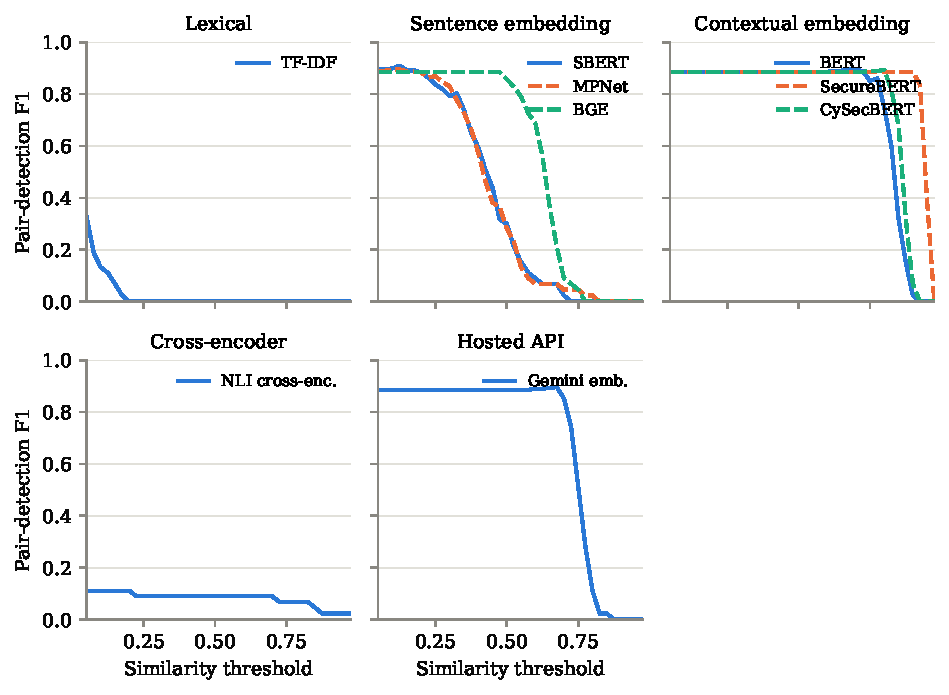
\includegraphics[width=0.78\textwidth]{figures/threshold_sweep}
\caption{Pair-detection F1 as a function of the decision threshold, computed
from the stored score matrices on the annotated scope, faceted by method
family. Eleven curves on shared axes cannot be distinguished by colour, and the
families are what the comparison is about.}
\label{fig:sweep}
\end{figure}

Figure~\ref{fig:sweep} separates representation quality from the choice of
operating point. Three observations stand out. First, the plateaus of BERT,
SecureBERT, and Gemini embeddings coincide with the all-positive baseline
(F1 $\approx$ 0.885) across most of the threshold range --- confirming that
their default-threshold results reflect saturation, not discrimination.
CySecBERT joins them, and the faceting makes the point sharper than a single
axis would: every member of the contextual-embedding panel shows the same
plateau, while no member of the sentence-embedding panel does.
Second, with an optimally chosen threshold Sentence-BERT becomes the
\emph{best} detector (F1 = 0.909 at $t=0.120$), despite being the worst
non-trivial one at its default operating point; MPNet and BGE reach 0.895 and
0.897 on the same basis, so the three sentence-embedding models are effectively
tied once their operating points are chosen properly. Their published default
entry thresholds are simply the wrong ones for cross-standard requirement
text. Choosing a
threshold on the same pairs the score is reported on inflates it, so the sweep
was repeated under 5-fold cross-validation with 20 repetitions: the threshold is
selected on four folds and scored on the fifth. Held-out F1 is
$0.903 \pm 0.021$, an optimism of only 0.006, because a single tuned parameter
over 107 points has little room to overfit.
Figure~\ref{fig:cvthreshold} shows the same comparison for every method with a
continuous score, together with the spread of the selected threshold itself. The
two panels carry different news: held-out F1 tracks the in-sample optimum closely
everywhere, but the threshold that produces it is stable only for some models.
Gemini embeddings settle on $0.658 \pm 0.023$ across all 100 fits, whereas
SecureBERT ranges over $0.265 \pm 0.375$ --- its folds disagree about the
operating point by more than the width of the useful range, which is the same
brittleness the sweep curve shows from a different angle.
Calibration gain is therefore real,
though Section~\ref{sec:prevalence} shows it is measured at a positive rate the
corpus does not share. Third,
the sharp cliffs on the right show how brittle threshold-based labelling is:
for SecureBERT the entire working range collapses within a few hundredths.
For practice this means thresholds must be calibrated per corpus and per
model --- fixed literature values do not transfer.

\begin{figure}[htbp]
\centering
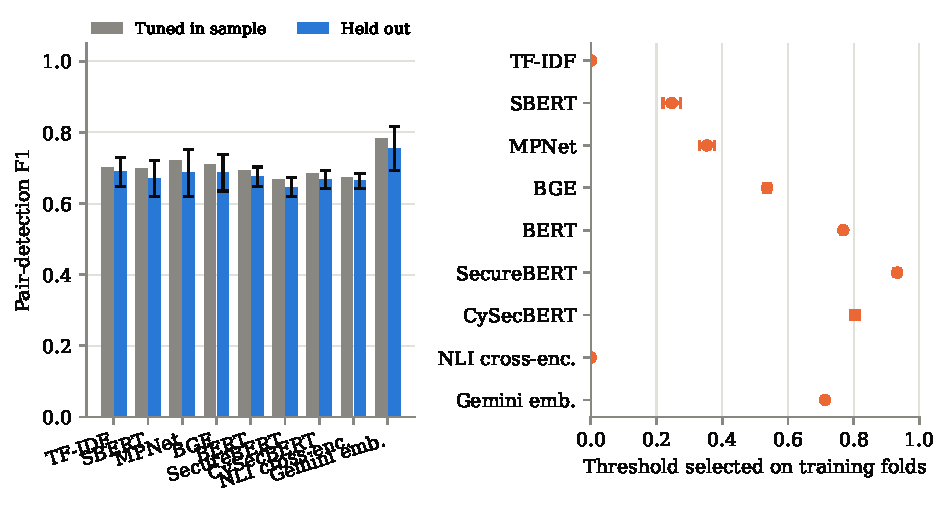
\includegraphics[width=\textwidth]{figures/cv_threshold}
\caption[Cross-validated threshold calibration]{Left: pair-detection F1 with the
threshold tuned on the same pairs it is scored on, against the held-out mean of
20 repeats of stratified 5-fold cross-validation (error bars, one standard
deviation). Right: the threshold each set of training folds selected.}
\label{fig:cvthreshold}
\end{figure}

\section{Corpus-level performance}\label{sec:prevalence}

Every figure reported so far describes the 107 pilot pairs, of which 85 are
related --- a positive rate of 79.4\%. That set was assembled purposively, so it
carries no inclusion probabilities and its precision cannot be reweighted to the
corpus it was drawn from. Because precision and F1 both move with the positive
rate, this matters: a method evaluated where four pairs in five are related is
being asked an easier question than the one it would face in use.

To measure rather than assume the difference, a stratified probability sample of
the full $69\times72$ space was drawn and annotated independently
(Section~\ref{sec:sampling}). Each pair carries a known inclusion probability, so
Horvitz--Thompson estimation recovers corpus-level quantities with correct
variance.

\paragraph{How common are related pairs?} The sample puts the corpus rate at
\textbf{12.4\%} (95\% CI [10.0, 15.0]) for any relationship, and \textbf{5.9\%}
(95\% CI [4.3, 7.7]) counting only equivalence, overlap and subsumption. Applied
to 4{,}968 candidates that implies roughly 617 and 295 related pairs
respectively. The pilot's 85 was never a measurement of this quantity --- it was
the number of pairs that study examined.

The unequal sampling fractions cost some precision of their own. With weights
ranging from 1.99 to 14.91, Kish's design effect is 1.49, so the 650 annotated
pairs carry the information of roughly 437 drawn with equal probability. Every
interval reported below already accounts for this, because the bootstrap
resamples within stratum.

\begin{table}[htbp]
\centering
\caption[Corpus-level detection performance]{Detection performance estimated over
all 4{,}968 candidate pairs from the weighted sample, at each method's shipped
operating point. Specificity is the fraction of unrelated pairs correctly
rejected. The final row is a classifier that labels every pair related.}
\label{tab:weighted}
\small
\begin{tabular}{lcccc}
\toprule
Method & Precision & Recall & Specificity & F1\\
\midrule
TF--IDF                 & 0.000 & 0.000 & 1.000 & 0.000\\
Keyword Jaccard         & 0.101 & 0.019 & 0.976 & 0.033\\
Sentence-BERT           & \textbf{0.905} & 0.061 & 0.999 & 0.115\\
MPNet                   & 0.696 & 0.057 & 0.997 & 0.106\\
BGE                     & 0.147 & 0.867 & 0.289 & \textbf{0.252}\\
BERT                    & 0.128 & 1.000 & 0.038 & 0.228\\
SecureBERT              & 0.124 & 1.000 & 0.000 & 0.221\\
CySecBERT               & 0.124 & 1.000 & 0.000 & 0.221\\
NLI cross-encoder       & 0.129 & 0.027 & 0.974 & 0.045\\
Gemini embeddings       & 0.124 & 1.000 & 0.000 & 0.221\\
Gemini LLM              & 0.121 & 0.886 & 0.092 & 0.214\\
\midrule
\emph{Label every pair related} & \emph{0.124} & \emph{1.000} & \emph{0.000} & \emph{0.221}\\
\bottomrule
\end{tabular}
\end{table}

\paragraph{The ranking inverts.} Table~\ref{tab:weighted} does not rearrange the
pilot ordering so much as contradict it. SecureBERT, CySecBERT and Gemini
embeddings reach specificity 0.000: across the weighted sample they reject no
unrelated pair at all, and their scores match the all-positive baseline to three
decimals. BERT, which led the pilot benchmark at detection F1 0.895, rejects
3.8\% of unrelated pairs. A paired bootstrap on the difference in F1 --- both
methods scored on the same resampled pairs, which is the comparison the overlap
of two marginal intervals does not make --- leaves four of the eleven methods
inside the baseline's interval: SecureBERT, CySecBERT and Gemini embeddings at
exactly zero difference, and the Gemini LLM at $-0.007$ [$-0.025$, 0.009]. BERT
sits ahead of the baseline by 0.007 [0.003, 0.011], a margin with no practical
content.

Sentence-BERT and MPNet move the other way. Both looked mediocre on the pilot set
(F1 0.300 and 0.283) and are the only methods here with precision of practical
interest: 0.905 and 0.696, meaning most of what they surface is genuinely
related. They pay for it with recall near 0.06. The NLI cross-encoder behaves
the same way from the other end of the design space --- precision 0.129 at recall
0.027 --- and BGE, alone among the sentence-embedding models, lands in the
saturated regime instead, flagging 87\% of the corpus.

That split runs along family lines, and it is the clearest structural finding
of the corpus view. The three models never trained for sentence similarity
(BERT, SecureBERT, CySecBERT) all saturate. Two of the three trained for it
(Sentence-BERT, MPNet) do the opposite and become too conservative to be useful.
Neither behaviour is about the model's size or its domain; both are about
whether its score distribution happens to straddle the threshold it inherited.

Sensitivity and specificity are properties of a classifier alone; precision also
depends on how common the positive class is. Fixing the first two therefore fixes
precision as a function of prevalence, plotted in
Figure~\ref{fig:precprev}. Three of the four methods shown lie on the diagonal
$\text{precision} = \text{prevalence}$, the locus of a classifier that carries no
information about the label: at the pilot's 0.79 they return 0.79, which reads as
strong performance, and at the corpus rate of 0.12 they return 0.12. Only
Sentence-BERT's curve stands away from the diagonal, and it is the separation
between curve and diagonal --- not the height of either --- that measures
discrimination.

\begin{figure}[htbp]
\centering
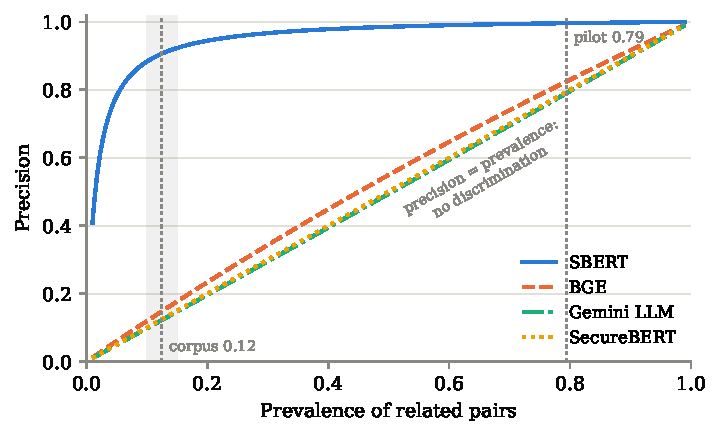
\includegraphics[width=0.78\textwidth]{figures/precision_vs_prevalence}
\caption[Precision as a function of prevalence]{Precision implied by each
method's estimated sensitivity and specificity as the share of related pairs
varies. Dotted lines mark the pilot set's positive rate and the corpus estimate;
the shaded band is the 95\% interval on the latter.}
\label{fig:precprev}
\end{figure}

\paragraph{How much of the collapse is the threshold?} Table~\ref{tab:weighted}
scores each method at the operating point Chapter~\ref{ch:prototype} shipped, and
those thresholds were chosen on the pilot set. Selecting a cut-off where 79\% of
pairs are related and then applying it where 12\% are confounds the method with
its calibration, so the comparison was repeated with the operating point selected
on the probability sample itself: weighted F1 maximised on four folds and scored
on the fifth, 20 repeats, stratified so every fold carries all three strata, with
the reported threshold the median of the 100 selections rather than the in-sample
optimum. Candidate cut-offs are quantiles of each method's own scores, since the
methods occupy very different ranges --- TF--IDF tops out at 0.14 while SecureBERT
never drops below 0.91, and a shared absolute grid would give one of them a
hundred candidate thresholds and the other three.

\begin{table}[htbp]
\centering
\caption[Corpus performance at a corpus-calibrated operating point]{Detection
performance when the threshold is selected on the probability sample instead of
the pilot set. Held-out F1 is the cross-validated mean; the gap to the point
estimate is the remaining optimism.}
\label{tab:calibrated}
\small
\begin{tabular}{lccccc}
\toprule
Method & Threshold & Precision & Recall & F1 & Held-out F1\\
\midrule
Gemini embeddings & 0.719 & \textbf{0.446} & 0.571 & \textbf{0.501} & 0.485\\
BGE               & 0.578 & 0.360 & 0.570 & 0.441 & 0.413\\
MPNet             & 0.325 & 0.336 & 0.611 & 0.434 & 0.405\\
Sentence-BERT     & 0.324 & 0.327 & 0.571 & 0.416 & 0.378\\
TF--IDF           & 0.017 & 0.281 & 0.367 & 0.319 & 0.285\\
BERT              & 0.824 & 0.233 & 0.477 & 0.313 & 0.289\\
CySecBERT         & 0.857 & 0.204 & 0.497 & 0.289 & 0.274\\
SecureBERT        & 0.939 & 0.178 & 0.508 & 0.264 & 0.252\\
NLI cross-encoder & 0.002 & 0.194 & 0.334 & 0.246 & 0.211\\
\midrule
\emph{Label every pair related} & --- & \emph{0.124} & \emph{1.000} & \emph{0.221} & ---\\
\bottomrule
\end{tabular}
\end{table}

The result changes the diagnosis (Figure~\ref{fig:calibgap}). At a threshold
fitted to the corpus, seven of the nine continuous methods clear the all-positive
baseline by a margin the paired bootstrap separates from zero. Gemini embeddings
lead at $+0.280$ [0.204, 0.362], with BGE at $+0.221$ [0.145, 0.295], MPNet at
$+0.213$ [0.146, 0.282] and Sentence-BERT at $+0.195$ [0.126, 0.267] behind it.
TF--IDF, BERT and CySecBERT beat it by 0.098, 0.093 and 0.068, intervals
excluding zero but only just. Two do not clear it at all: SecureBERT
($+0.043$, [$-0.009$, 0.095]) and the NLI cross-encoder
($+0.025$, [$-0.049$, 0.098]).

The top of that ranking is a four-way tie rather than a winner. Measured against
the leader, BGE ($-0.060$, [$-0.161$, 0.045]), MPNet ($-0.067$, [$-0.160$,
0.019]) and Sentence-BERT ($-0.085$, [$-0.184$, 0.015]) all have intervals
containing zero, so the honest statement is that a hosted commercial embedding
and three freely available local models cannot be told apart on this task. That
matters practically: the best local model matches the paid one within the
resolution this sample supports.

What collapsed in Table~\ref{tab:weighted}, then, was mostly calibration rather
than representation. The embedding spaces do carry enough signal to reject
unrelated pairs; the thresholds inherited from a 79\%-positive development set
did not let them. That is a sharper version of the same warning: the cost of a
development set at the wrong base rate is not a mild optimism in the reported
score, it is an operating point that turns a usable model into a constant
function. SecureBERT is the exception, and the informative one --- its scores
occupy a band 0.06 wide across the entire corpus, so no threshold placed anywhere
in that band separates the classes. CySecBERT, adapted to the same domain from a
different base model by a different group, is the near-exception: it recovers
enough range to clear the baseline by 0.068, but still finishes below plain BERT.
Two independent attempts at cybersecurity domain adaptation both end up worse
than the general-purpose model they were built from, which is a stronger
statement than either could make alone.

\begin{figure}[htbp]
\centering
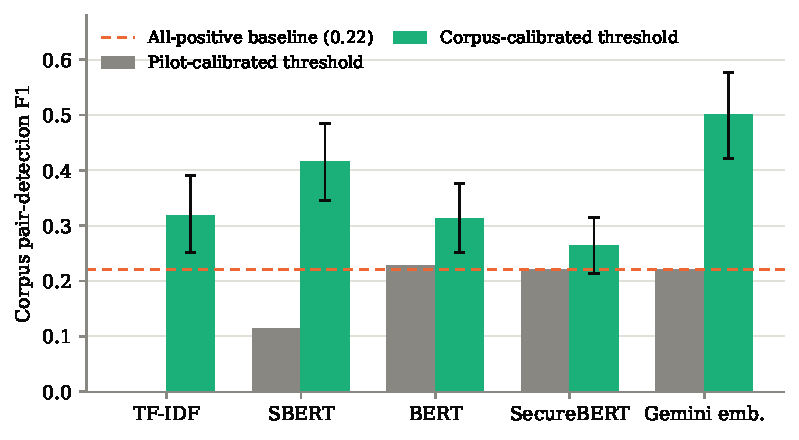
\includegraphics[width=0.82\textwidth]{figures/calibration_gap}
\caption[Effect of recalibrating the operating point]{Corpus pair-detection F1 at
the shipped, pilot-calibrated threshold against a threshold cross-validated on
the probability sample. Error bars are stratified bootstrap 95\% intervals.}
\label{fig:calibgap}
\end{figure}

\paragraph{What this supports.} Even recalibrated, no method here supports an
automated accept/reject decision: the best F1 is 0.50, with precision 0.45, so
more than half of what the system proposes is wrong. The defensible use is the
one Section~\ref{sec:discussion} describes --- ranking candidates for a human
reviewer --- and the choice of configuration depends on which end of the trade-off
matters. Sentence-BERT at its shipped threshold surfaces few pairs but is right
about nine times in ten; Gemini embeddings recalibrated recover 57\% of the
related pairs at under half precision. Neither removes the reviewer.

\section{Relationship classification}\label{sec:classresults}

Detecting that two provisions relate is only half the task; compliance work
needs to know \emph{how} they relate. Table~\ref{tab:classification}
summarises classification performance.

\begin{table}[htbp]
\centering
\caption{Relationship classification over all 107 annotated pairs, five-label
scheme (subsumption directions merged). CIs are bootstrap 95\% intervals.}
\label{tab:classification}
\small
\begin{tabular}{lccc}
\toprule
Method & Accuracy & Macro-F1 & Macro-F1 95\% CI\\
\midrule
TF--IDF            & 0.215 & 0.086 & [0.053, 0.128]\\
Keyword Jaccard    & 0.224 & 0.179 & [0.059, 0.288]\\
Sentence-BERT      & 0.224 & 0.099 & [0.064, 0.137]\\
MPNet              & 0.224 & 0.100 & [0.064, 0.140]\\
BGE                & 0.243 & 0.149 & [0.098, 0.199]\\
BERT               & 0.411 & 0.172 & [0.114, 0.234]\\
SecureBERT         & 0.028 & 0.011 & [0.000, 0.025]\\
CySecBERT          & 0.196 & 0.087 & [0.057, 0.118]\\
NLI cross-encoder  & 0.215 & 0.102 & [0.054, 0.164]\\
Gemini embeddings  & \textbf{0.477} & \textbf{0.279} & [0.150, 0.388]\\
Gemini LLM         & 0.187 & 0.088 & [0.052, 0.127]\\
\bottomrule
\end{tabular}
\end{table}

\begin{figure}[htbp]
\centering
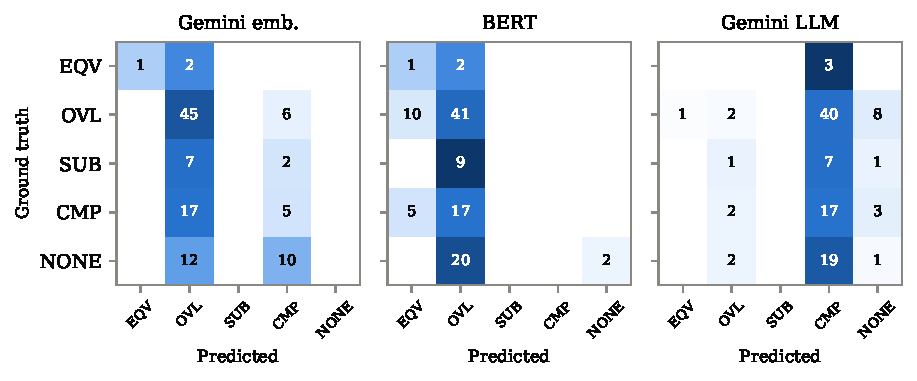
\includegraphics[width=\textwidth]{figures/confusion_matrices}
\caption{Row-normalised confusion matrices (counts printed) for the most
instructive methods, one per family. EQV = equivalence, OVL = overlap, SUB = subsumption,
CMP = complementarity, NONE = no relation.}
\label{fig:confusion}
\end{figure}

Classification is where every method struggles. The best result --- Gemini
embeddings at 0.477 accuracy and 0.279 macro-F1 --- would still mislabel every
second pair. The comparison that matters is against the trivial classifier
that assigns the majority label to everything: \textsc{Overlap} accounts for
51 of the 107 pairs, so always predicting it yields 0.477 accuracy. The best
method matches that figure exactly and none exceeds it. The same baseline
scores 0.129 macro-F1, which four methods do beat --- keyword Jaccard, BGE, BERT
and Gemini embeddings --- so the methods are not uniformly worthless; but the
headline conclusion has to be stated plainly. On the five-label task, none of the eleven methods learns the
distinction the task is about. The confusion matrices in
Figure~\ref{fig:confusion} show how each one fails:

\begin{itemize}
  \item \textbf{Gemini embeddings} funnel most predictions into
  \textsc{Overlap}. That matches the majority class (hence the comparatively
  high accuracy) and yields reasonable per-class scores for \textsc{Overlap}
  (F1 = 0.65) and \textsc{Equivalence} (precision 1.00 at recall 0.33), but
  \textsc{Subsumption} and \textsc{No relation} are never predicted
  correctly.
  \item \textbf{BERT} spreads slightly more but shows the same collapse;
  \textsc{Complementarity} and \textsc{Subsumption} both go to zero.
  \item \textbf{The Gemini LLM} is the only method that predicts labels from
  provision content rather than a score band, and it does recognise
  complementarity (recall 0.59) --- but it heavily overuses it, pushing 41 of
  the 51 \textsc{Overlap} pairs into \textsc{Complementarity} and ending with
  the lowest accuracy of the non-degenerate methods. Notably, it also assigns
  a relation to 20 of the 22 annotated negatives.
  \item \textbf{SecureBERT}'s uniform \textsc{Equivalence} output produces
  0.028 accuracy --- exactly the 3 equivalence pairs in the ground truth.
  \item \textbf{The NLI cross-encoder} is the only method that predicts
  \textsc{Subsumption} at all. Over the full corpus it emits 123 subsumption
  labels where every other method emits none, because every other method scores
  pairs with a symmetric function and direction is not recoverable from one. Its
  macro-F1 of 0.102 is nonetheless unremarkable, and the reason is instructive:
  it is extremely conservative, flagging 142 of 4{,}968 pairs, so it reaches the
  directional label on too few pairs to score well. The capability is real and
  the recall is not. This is the one structural gap in the taxonomy that a
  different architecture --- rather than a better-calibrated threshold --- does
  close, which is why it is worth reporting despite the weak headline number.
\end{itemize}

Two error examples illustrate the pattern. Provision 5.3-11 of \standardA{}
(inform the user that a security update is required, with its risks) and
provision 5.3.1-2.2 of \standardB{} (proactively inform end-users of
security-relevant updates with clear explanations) are annotated
\textsc{Equivalence}; Gemini embeddings scored the pair into the
\textsc{Overlap} band --- a near-miss that a human reviewer would accept as a
shortlist hit. By contrast, the Gemini LLM labelled the pair of provision
5.1-1 (unique per-device passwords) and provision 5.2.2-1 (evaluate access
control frameworks for APIs, models, and data) as \textsc{Complementarity}
where the annotation says \textsc{Overlap}: both provisions govern
authentication-related access control, but the model read the difference in
system layer as a difference in objective. The boundary between overlap and
complementarity is exactly where the annotation itself is hardest, a point
the validation study below quantifies.

\section{Coverage and gaps}\label{sec:coverage}

The preceding sections measure how often a method is right. This one asks what
the method actually says about the two standards, which is the question a
compliance practitioner brings to a mapping exercise: which provisions of
\standardA{} have a counterpart in \standardB{}, and which have none. The
manual study closest to this one~\cite{djebbar2023comparative} reports exactly
that --- a coverage statement and an explicit list of unmapped requirements ---
so producing the same two artefacts automatically is the fairest way to show
what the automation delivers.

Everything in this section is a prediction from a single method, the
best-scoring one at its corpus-calibrated operating point, and its precision at
that point is 0.446 with a 95\% interval of [0.362, 0.535]. Roughly half of
what follows is therefore wrong. The section is included because a shortlist
with a known error rate is a usable artefact and a mapping with an unknown one
is not, but nothing here carries the standing of the estimates in
Section~\ref{sec:prevalence}.

At its calibrated threshold the method flags 797 of the 4{,}968 candidate pairs,
16.0\% of the space, against an estimated true prevalence of 12.4\%
[10.0\%, 15.0\%]. It over-predicts, which is what a threshold chosen to maximise
F1 at a low base rate should do: recall is worth more than precision when the
output is a shortlist for human review.

\begin{figure}[htbp]
  \centering
  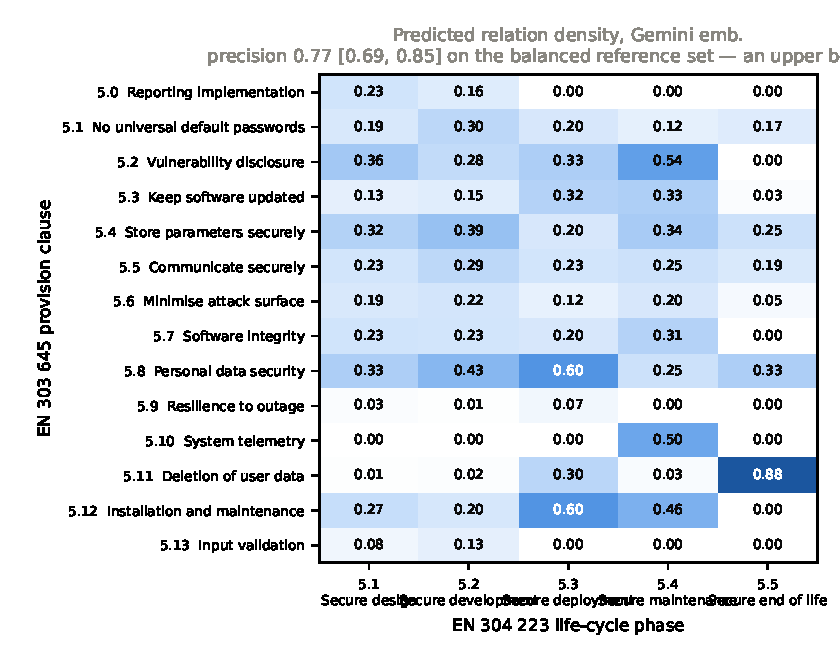
\includegraphics[width=0.82\linewidth]{figures/coverage_heatmap.pdf}
  \caption{Predicted relation density by clause. Each cell is the share of
  provision pairs in that clause block flagged as related by Gemini embeddings
  at the corpus-calibrated threshold of 0.719. These are predictions, not
  verified relations: the method's precision at this operating point is 0.446
  [0.362, 0.535].}
  \label{fig:coverage}
\end{figure}

Figure~\ref{fig:coverage} shows where the predicted relations concentrate. The
density is uneven in a way that follows the structure of the two documents
rather than the behaviour of the model.

The gap side is the more informative one, and it is the part a similarity
threshold can state cleanly. Eight of the 69 \standardA{} provisions and five
of the 72 \standardB{} provisions receive no predicted counterpart at all;
Table~\ref{tab:unmapped} lists them. A gap here is a weaker claim than a gap in
a manual study: it means the method found nothing, not that nothing is there,
and at a recall well below one the two are different statements. The list is
useful in the direction that a false gap is cheap to check --- an analyst reads
thirteen provisions --- and expensive to miss.

\begin{table}[htbp]
  \centering
  \caption{Provisions with no predicted counterpart in the other standard, at
  the corpus-calibrated operating point. Absence of a prediction is not evidence
  of absence of a relation; the method's recall at this threshold is below one.}
  \label{tab:unmapped}
  \small
  % Generated by src.evaluation.coverage -- do not edit by hand.
\begin{tabular}{@{}llp{0.60\linewidth}@{}}
\toprule
Standard & Provision & Requirement \\
\midrule
EN 303 645 & 5.1-2A & Passwords should not be used for machine-to-machine authentication. Using human-memorable p\textbackslash{}ldots \\
 & 5.3-15A & For devices that cannot have their software updated, the consumer IoT device should be isol\textbackslash{}ldots \\
 & 5.5-3 & Cryptographic algorithms and primitives should be replaceable. \\
 & 5.5-4 & Access to consumer IoT device functionality via a network interface in the initialized stat\textbackslash{}ldots \\
 & 5.6-4B & Debug interfaces that are physical ports should be physically protected by the device. \\
 & 5.6-6 & Code should be minimized to the functionality necessary for the consumer IoT device to oper\textbackslash{}ldots \\
 & 5.9-2 & Consumer IoT devices should remain operating and locally functional in the case of a loss o\textbackslash{}ldots \\
 & 5.9-3 & The consumer IoT device should connect to networks in an expected, operational and stable s\textbackslash{}ldots \\
\midrule
EN 304 223 & 5.1.1-1.1 & AI security training shall be tailored to the specific roles and responsibilities of staff\textbackslash{}ldots \\
 & 5.1.2-1.1 & Where the Data Custodian is part of a Developer's organization, they shall be included in i\textbackslash{}ldots \\
 & 5.1.3-1.3 & System Operators shall apply controls to risks identified through the analysis based on a r\textbackslash{}ldots \\
 & 5.2.3-3 & Developers and System Operators shall re-run evaluations on released models that they inten\textbackslash{}ldots \\
 & 5.2.5-2 & System Operators shall conduct testing prior to the system being deployed with support from\textbackslash{}ldots \\
\bottomrule
\end{tabular}

\end{table}

The full predicted mapping --- all 797 pairs with their scores --- is given in
Appendix~\ref{app:mapping}. Both the table above and that appendix are
generated directly from the evaluation outputs, so neither can drift from the
numbers reported here.

\section{Ground-truth validation}\label{sec:agreementresults}

A reference set is only as good as the consistency of the judgements behind it.
The pilot pairs were mixed unmarked into the annotation stream for the
probability sample, so re-labelling them was blind: at the time of judging, there
was no way to tell a pilot pair from a newly sampled one. Comparing the two label
sets afterwards gives an agreement figure against annotations that two authors
reviewed months earlier.

\begin{table}[htbp]
\centering
\caption[Reference-set agreement against the pilot and the LLM contrast]{%
Agreement of the annotated reference sample with the earlier author-reviewed
pilot labels, against the same statistic computed for the evaluated LLM on two
runs over identical input.}
\label{tab:agreement}
\small
\begin{tabular}{lccccc}
\toprule
 & & \multicolumn{2}{c}{Six labels} & \multicolumn{2}{c}{Related vs.\ not}\\
\cmidrule(lr){3-4}\cmidrule(lr){5-6}
Comparison & $n$ & Agreement & $\kappa$ & Agreement & $\kappa$\\
\midrule
Reference sample vs.\ author-reviewed pilot & 107 & 0.61 & 0.40 & 0.82 & 0.51\\
Evaluated LLM vs.\ itself, identical input & 4\,968 & 0.69 & 0.02 & 0.81 & $-$0.03\\
\bottomrule
\end{tabular}
\end{table}

Agreement with the pilot reaches $\kappa = 0.51$ on the detection decision and
$\kappa = 0.40$ on the six-label scheme --- moderate on both counts on the
Landis--Koch scale~\cite{landis1977kappa}. This is weaker than it looked partway
through annotation, when the 47 pilot pairs reached so far gave 0.68 and 0.44;
the figures above are over all 107 and are the ones that should be read. A
reference set at $\kappa = 0.51$ on its central decision is usable for comparing
methods against each other, since every method is scored against the same labels,
but it is not precise enough to certify an absolute performance level, and the
method rankings in Section~\ref{sec:prevalence} should be read with that ceiling
in mind.

Disagreements are not scattered across the label space. They cluster on the
overlap/complementarity boundary, which Section~\ref{sec:threats} identifies as
the least determinate distinction in the taxonomy, and on the general-process
provisions covered by the codebook amendment recorded during annotation. Recorded
confidence tracks them: pairs marked confidence 3 agree with the pilot 77\% of
the time against 46\% for confidence 2. The scale collapsed in practice to those
two values --- no pair was recorded at 1, 4 or 5 --- so this is a two-level
contrast rather than a calibration curve, but it does show the field carries
information rather than noise.

The second row of Table~\ref{tab:agreement} is the more instructive one. The
evaluated LLM was run twice at temperature 0 over byte-identical prompts. The two
runs agree on 69\% of pairs --- \emph{higher} raw agreement than the human comparison
--- yet reach $\kappa = 0.02$. The explanation is that the model assigns
\textsc{Complementarity} to 81\% of all pairs, so two runs coincide frequently
without either run carrying information. Raw agreement rewards a degenerate
marginal; $\kappa$ does not. This is why the reliability of an annotation source
cannot be read off its agreement percentage, and it is the clearest single
demonstration in this study of why the LLM classifier's headline scores should
not be taken at face value.

Recorded annotation confidence behaves as intended: pairs marked confidence~3
agree with the pilot 82\% of the time ($n = 22$), against 48\% for those marked
confidence~2 ($n = 25$). The field predicts where judgement is contestable, so
it is retained rather than discarded.

\section{Efficiency and interpretability}\label{sec:efficiency}

\begin{table}[htbp]
\centering
\caption[Wall-clock runtime per stage]{Wall-clock runtime per stage on an
8\,GB Apple silicon laptop, including model loading but not the one-off model
download (about 2\,GB in total). Embedding stages use the Metal backend. Gemini
stages run through the batch API; their end-to-end time is dominated by queueing
(minutes to hours) rather than computation.}
\label{tab:runtime}
\small
\begin{tabular}{lr}
\toprule
Stage & Runtime\\
\midrule
Provision extraction (both PDFs) & 0.9 s\\
TF--IDF + keyword mapping        & 3.5 s\\
Sentence-BERT mapping            & 1.8 s\\
MPNet mapping                    & 3.9 s\\
BGE mapping                      & 3.9 s\\
BERT mapping                     & 4.2 s\\
SecureBERT mapping               & 5.7 s\\
CySecBERT mapping                & 3.9 s\\
NLI cross-encoder (9{,}936 forward passes) & 327 s\\
Gemini embeddings                & API batch\\
Gemini LLM classification (4{,}968 prompts) & API batch\\
Evaluation                       & 1.4 s\\
Corpus estimation (bootstrap + calibration) & 612 s\\
\bottomrule
\end{tabular}
\end{table}

Every local method runs in seconds or minutes on commodity hardware
(Table~\ref{tab:runtime}); by comparison, drafting and reviewing the 107 pilot
pairs occupied several working days even with LLM assistance, and the 650
sampled pairs took several times that again. The cost structure separates the
two architectures cleanly. A bi-encoder embeds each provision once, so the work
is linear in the 141 provisions and the 4{,}968 similarities are a single matrix
product --- which is why every embedding stage finishes in under six seconds. A
cross-encoder must run the model once per pair per direction, so its work is
quadratic in the provisions: 9{,}936 forward passes and 327 seconds, roughly
sixty times the cost of the slowest bi-encoder for the same corpus. On this pair
of standards that is affordable; on a pair ten times larger it would not be.

Interpretability differs more than runtime: the keyword baseline can show
\emph{which} terms matched, embedding methods offer only an opaque score, the
cross-encoder additionally reports which direction the entailment ran, and the
LLM can produce a textual rationale on request --- though its rationale quality
was not separately evaluated here.

\section{Discussion}\label{sec:discussion}

\paragraph{RQ1 --- feasibility and limits.}
Automated methods can reliably \emph{shortlist} related provisions: the better
embedding models place genuinely related pairs high in their rankings, and
with a calibrated threshold Sentence-BERT reaches detection F1 above 0.9 on
the annotated scope --- although, as Section~\ref{sec:prevalence} shows, that
figure reflects the benchmark's high positive rate more than deployable
accuracy. Identifying the \emph{type} of relationship is a
different matter. The best classification result (macro-F1 0.279) is far from
usable autonomy, and structural limits are visible: the
overlap/complementarity boundary requires judging \emph{objectives}, not
surface meaning. The fundamental limitation is that a scalar similarity
collapses precisely the distinctions the taxonomy is designed to capture.

One of those limits turns out to be architectural rather than fundamental.
Symmetric similarity cannot express directional subsumption --- but the NLI
cross-encoder, which asks a directional question by construction, predicts 123
subsumption relations where the other ten methods predict none. It does so at
too low a recall to be useful on its own, so the practical conclusion is
unchanged; the theoretical one is not. The distinction the taxonomy needs is
reachable, just not by the family of methods that dominates this literature.

\paragraph{RQ2 --- method comparison.}
No method family wins outright; they fail differently, and with three models
in each of the two embedding families the failures separate by family rather
than by model. Lexical baselines are precise but nearly blind (recall $\leq$
0.07). Contextual embeddings saturate: anisotropy makes their cosine scores
unusable without calibration, and all three sit at the bottom of the calibrated
ranking. Domain pretraining makes this worse rather than better, and that now
rests on two independent models --- SecureBERT and CySecBERT, built by different
groups from different base models --- both of which finish below the plain BERT
they were adapted from. The intuition that cybersecurity vocabulary is the
missing ingredient is not merely unsupported; it is contradicted twice.

The sentence-embedding models are the strongest local family once calibrated,
and they are mutually indistinguishable: BGE 0.441, MPNet 0.434 and
Sentence-BERT 0.416, with paired intervals that all contain zero against the
leader. Gemini embeddings top the table at 0.501 and give the best label quality
overall (macro-F1 0.279, accuracy 0.477), but the paired bootstrap cannot
separate them from any of the three free local models --- so the practical answer
to whether the paid model is needed is no, not at the resolution this sample
supports. The cross-encoder buys direction at roughly sixty times the compute
and a recall too low to exploit it. The prompted LLM is the only method with
non-trivial recall on complementarity but over-predicts it massively.

The pilot and corpus views disagree about which method to prefer, and where they
disagree the corpus view should win. Once the operating point is fitted to the
corpus, four methods lead and the paired bootstrap separates none of them:
Gemini embeddings, BGE, MPNet and Sentence-BERT. Since accuracy does not decide
between them, practical grounds do. All three local models run in under four
seconds with no per-query cost and reproduce bit-identically across runs,
whereas the Gemini embeddings depend on a hosted model that can change under the
same name --- and the LLM replicate of Section~\ref{sec:agreementresults} shows
what hosted non-determinism costs. Calibrated BGE or MPNet for ranking, plus
human labelling of the shortlist, is the defensible configuration; the paid
model earns its place only where the marginal 0.06 F1 it may or may not carry is
worth the loss of reproducibility.

\paragraph{RQ3 --- automated versus human mapping.}
Against the author-reviewed reference, automation is dramatically faster
(seconds versus days) and consistent, but its label agreement
(at best 46\%) remains far below what compliance documentation requires.
These findings support the same conclusion Bar-Haim et
al.~\cite{barhaim2023cloud} reached for control mapping: automated compliance
mapping is a decision-support technology. Concretely, the evidence here
supports a workflow where an embedding model ranks all 4{,}968 pairs, a
human reviews the top of the ranking, and the relationship label is always
assigned by the human.

\section{Threats to validity}\label{sec:threats}

\paragraph{Construct validity.} The six-label taxonomy compresses a
continuum of relationships between requirements into discrete classes; the
overlap/complementarity boundary in particular is partly a judgement call.
Section~\ref{sec:agreementresults} puts a number on the cost: agreement on the
binary related/unrelated question reaches $\kappa = 0.51$, and resolving
\emph{which} of the six relations holds falls to $\kappa = 0.40$, so the typed
labels are the noisier construct and the classification results in
Section~\ref{sec:classresults} are measured against a correspondingly noisier
target.

\paragraph{Internal validity.} Both reference sets were drafted with LLM
assistance, which risks favouring LLM-family methods. Three things bound the
risk. The drafting model (Claude) belongs to a different family from the
evaluated ones (Gemini); the pilot's 107 pairs were reviewed by the authors; and
the evaluated LLM performed \emph{worst} of the non-degenerate methods, so the
circularity, if any, did not manifest as an advantage. The probability sample was
not author-reviewed pair by pair, and its reliability rests instead on the blind
comparison with the reviewed pilot reported in
Section~\ref{sec:agreementresults}. Fixed shared thresholds avoid per-method
tuning bias; the sweep and the cross-validated calibration show what tuning
would and would not change.

\paragraph{Statistical conclusion validity.} Three limits constrain how far the
numbers can be pushed. First, the pilot-set intervals in Figure~\ref{fig:cis}
overlap widely across the stronger methods; with 107 pairs, and with
\textsc{Equivalence} supported by only three of them, the ranking between
neighbouring methods on that set is not established. Corpus-scale comparisons are
made instead with a paired bootstrap on the difference, which is the test that
matches the design, and only differences whose interval excludes zero are
reported as orderings. Second, \textsc{Equivalence} does not occur in the
probability sample at all, so no weighted per-class estimate exists for it and the
classification results remain confined to the pilot set. Third, the corpus
operating points are selected by cross-validation on the same sample they are
scored on. The residual optimism is measured rather than assumed --- 0.016 for
Gemini embeddings, 0.048 for Sentence-BERT --- and is small relative to the gap
between those methods and the baseline, but the point estimates in
Table~\ref{tab:calibrated} sit slightly above what a fully independent test set
would give.

\paragraph{External validity.} Results cover one standard pair and specific model
versions; hosted models additionally evolve over time, and
\texttt{gemini-2.5-flash-lite} is scheduled for retirement in October 2026, after
which the LLM results here cannot be reproduced exactly. Generalisation to other
standards or model generations is plausible for the structural findings
(anisotropy, similarity-versus-taxonomy mismatch) but must be assumed with
caution for the specific numbers. The prevalence gap between the two reference
sets is itself the clearest warning: a benchmark assembled by looking for
interesting pairs measured something the deployed setting does not share.
